\documentclass[../main.tex]{subfiles}
\graphicspath{{\subfix{../images/}}}

\begin{document}

Στα παρακάτω σχήματα φαίνονται τρις σημαντικές μετρικές που καταγράφαμε κατά την
διάρκεια της εκπαίδευσης.

Πρώτη είναι η μετρική \textbf{Accuracy} που μας δείχνει πόσο συχνά οι προβλέψεις
του νευρωνικού δικτύου είναι σωστές.

Δεύτερη είναι η μετρική \textbf{Loss} και πιο συγκεκριμένα στα σχήματα
\ref{mfcc_loss} και \ref{spectogram_loss} χρησιμοποιήσαμε την \textit{Binary
	crossentropy loss function} η οποία υπολογίζει πόσο απέχει η πρόβλεψη του
νευρωνικού από την πραγματική τιμή μέσω της παρακάτω συνάρτησης
\ref{eq:binary_crossentropy}.

\begin{equation}\label{eq:binary_crossentropy}
	\mathrm{Loss} = - \frac{1}{\mathrm{output \atop size}} \sum_{i=1}^{\mathrm{output \atop size}} y_i \cdot \mathrm{log}\; {\hat{y}}_i + (1-y_i) \cdot \mathrm{log}\; (1-{\hat{y}}_i)
\end{equation}

Τελευταία μετρική είναι η \textbf{Recall} την οποία θεωρήσαμε πολύ σημαντική για
το συγκεκριμένο πρόβλημα, καθώς μας δείχνει το ποσοστό των σωστά
κατηγοροποιημένων ατόμων με πρόβλημα, από το σύνολο όλων αυτών τον ατόμων
(ιδανικά θα θέλαμε να έχουμε 100\% recall, δηλαδή να μπορούμε να εντοπίσουμε
κάθε άτομο με καρδιακό πρόβλημα).

\subsection{Χρήση MFCC}

Με την χρήση των MFCC ως είσοδο στο νευρωνικό το accuracy σταθεροποιείται κοντά
στο 81\%, ενώ το validation\_loss έχει αρκετή απόκλιση από το loss και κυμαίνετε
ανάμεσα στο 0.4 με 0.5. Το recall έχει δραματικές μεταβολές από εποχή σε εποχή
κάτι που θα εξηγηθεί παρακάτω, με μια μέση τιμή 45\% μετά την
40\textsuperscript{στη} εποχή.

\begin{figure}[H]
	\center
	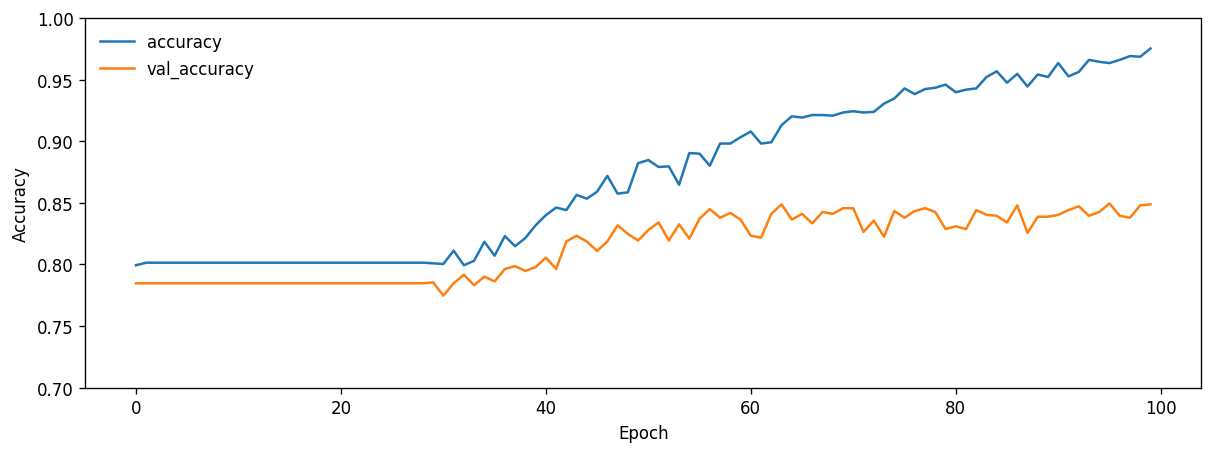
\includegraphics[width=\textwidth]{../images/mfcc_accuracy.png}
	\caption{Accuracy νευρωνικού δικτύου ανά εποχή με χρήση \textbf{MFCCs} ως
		είσοδο}
	\label{mfcc_accuracy}
\end{figure}
\begin{figure}[H]
	\center
	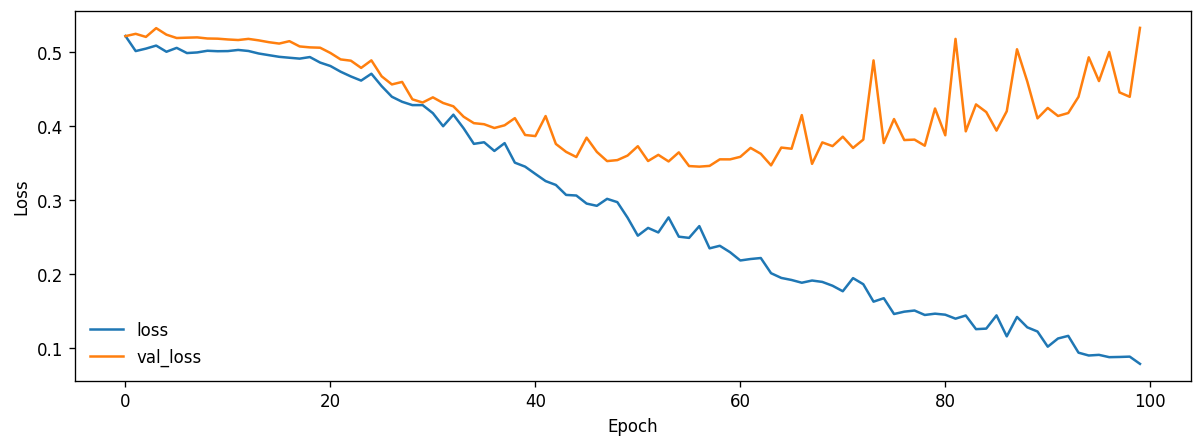
\includegraphics[width=\textwidth]{../images/mfcc_loss.png}
	\caption{Loss νευρωνικού δικτύου ανά εποχή με χρήση \textbf{MFCCs} ως
		είσοδο}
	\label{mfcc_loss}
\end{figure}
\begin{figure}[H]
	\center
	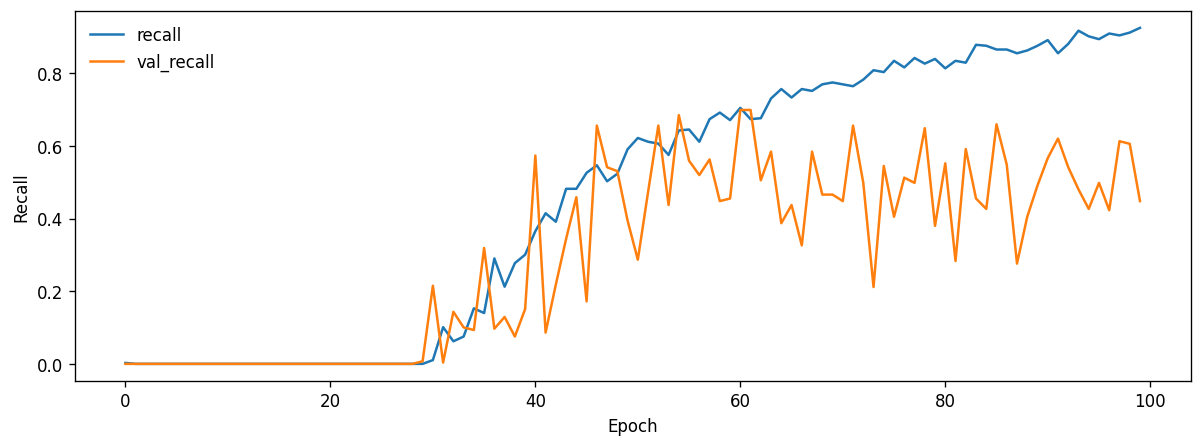
\includegraphics[width=\textwidth]{../images/mfcc_recall.png}
	\caption{Recall νευρωνικού δικτύου ανά εποχή με χρήση \textbf{MFCCs} ως
		είσοδο}
	\label{mfcc_recall}
\end{figure}


\subsection{Χρήση Mel spectogram}

Όταν χρησιμοποιήσαμε τα mel σπεκτογράμματα ως είσοδο στο νευρωνικό δίκτυο,
είδαμε ελαφρώς καλύτερα αποτελέσματα. Αφού πλέον η ακρίβεια σταθεροποιείται στο
86\% και το validation\_loss δεν απέχει τόσο από το loss με μέση τιμή κάτω από
0.35. Όσο αναφορά το recall, έχουμε κι εδώ μεγάλες μεταβολές από εποχή σε εποχή
με την τιμή να βρίσκετε γύρω από το 57\%.

\begin{figure}[H]
	\center
	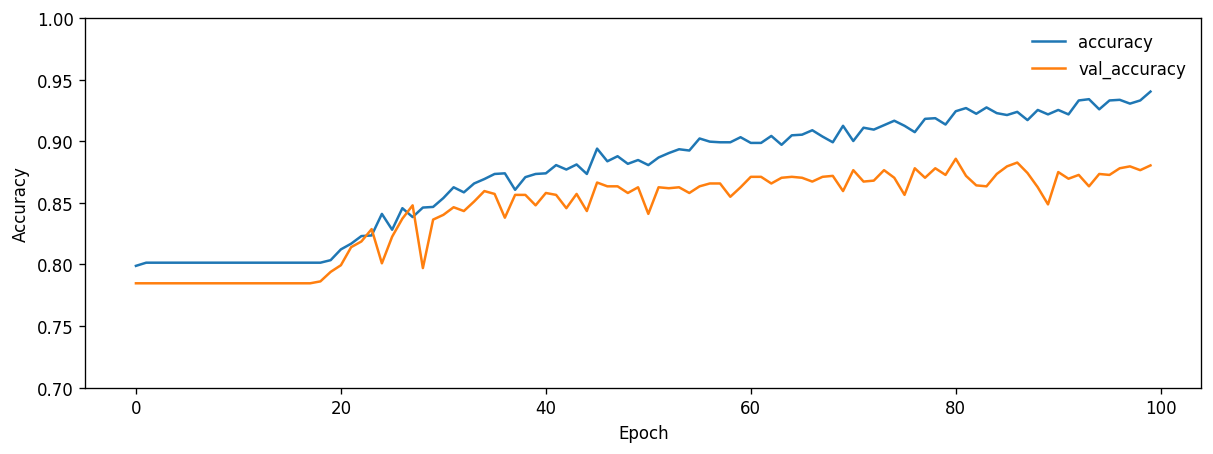
\includegraphics[width=\textwidth]{../images/spectogram_accuracy.png}
	\caption{Accuracy νευρωνικού δικτύου ανά εποχή με χρήση \textbf{spectogram} ως
		είσοδο}
	\label{spectogram_accuracy}
\end{figure}
\begin{figure}[H]
	\center
	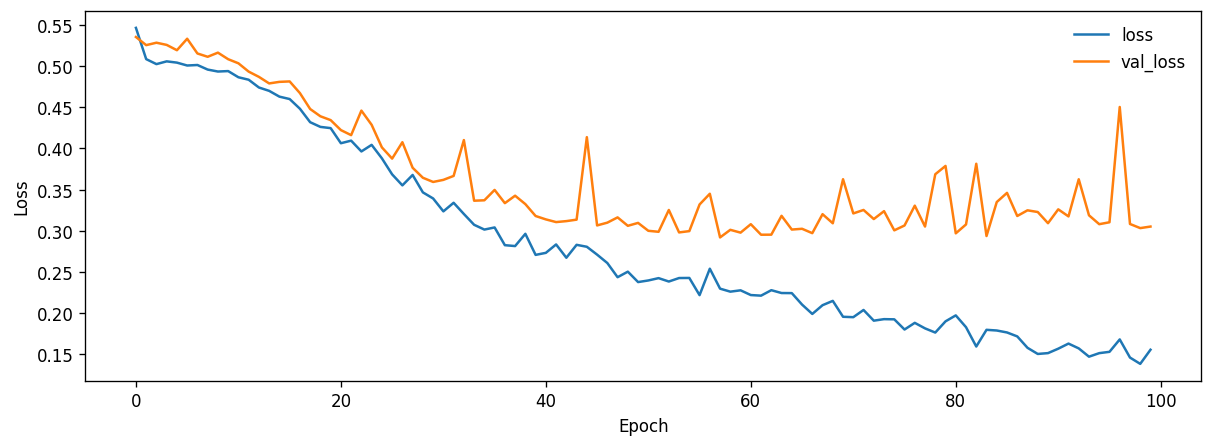
\includegraphics[width=\textwidth]{../images/spectogram_loss.png}
	\caption{Loss νευρωνικού δικτύου ανά εποχή με χρήση \textbf{spectogram} ως
		είσοδο}
	\label{spectogram_loss}
\end{figure}
\begin{figure}[H]
	\center
	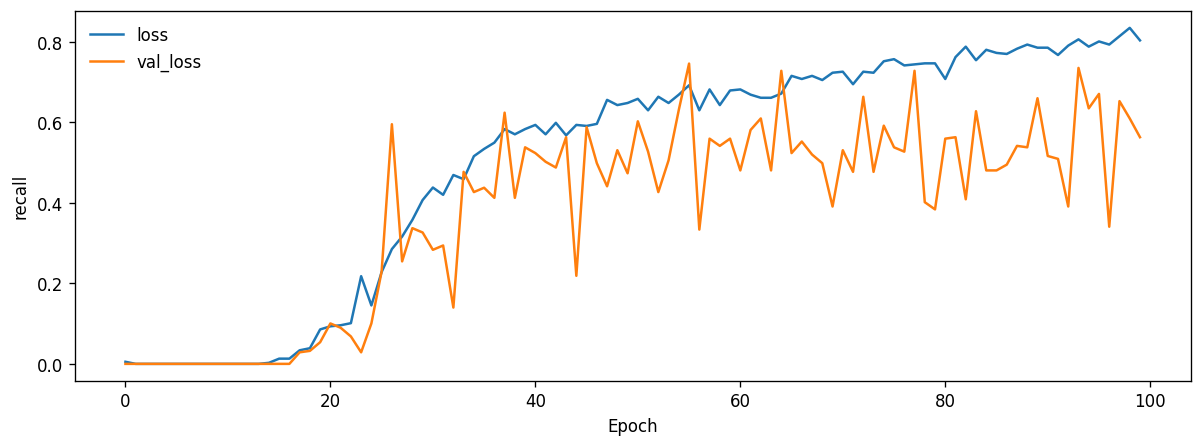
\includegraphics[width=\textwidth]{../images/spectogram_recall.png}
	\caption{Recall νευρωνικού δικτύου ανά εποχή με χρήση \textbf{spectogram} ως
		είσοδο}
	\label{spectogram_recall}
\end{figure}

\subsection{Συμπεράσματα}

Όπως είδαμε παραπάνω η καλύτερη προσπάθεια μας είχε 86\% accuracy με 57\% recall
όμως ακόμα κι αυτή η προσπάθεια δεν είναι ικανοποιητική λόγω των άνισων
δεδομένων. Τα δείγματα που παρείχε η Physionet \cite{physionet} ήταν συνολικά
3228 από τα οποία μόνο τα 665 (20\%) ήταν από ανθρώπους με καρδιοπάθεια.
Αυτό σημαίνει ότι ακόμα κι ένα νευρωνικό που θα κατηγοροποιούσε όλα τα δείγματα
ως 0 (δηλαδή χωρίς καρδιοπάθεια) θα είχε accuracy περίπου 80\% αλλά με 0\%
recall. Αυτή είναι και η αιτία που βλέπουμε και τις μεγάλες μεταβολές από εποχή
σε εποχή στο recall καθώς το δίκτυο έχει την τάση να κατηγοριοποιεί κάθε δείγμα
ως άτομο χωρίς καρδιοπάθεια λόγω της αριθμητικής υπεροχής αυτών τον ατόμων στα
δείγματα.

\end{document}
